\begin{figure}[H]
    \centering
    \begin{subfigure}{0.45\textwidth}
        \centering
        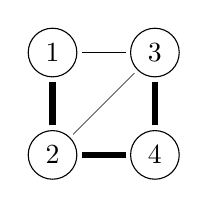
\begin{tikzpicture}[scale=1, every node/.style={circle,draw,minimum size=5mm}]
            \node (n0) at (0,1.3) {1};
            \node (n1) at (0,0) {2};
            \node (n2) at (1.3,1.3) {3};
            \node (n3) at (1.3,0) {4};
            \draw[line width=0.8mm, black] (0,0.375) -- (0,0.93);
            \draw[line width=0.8mm, black] (1.3,0.375) -- (1.3,0.93);
            \draw[line width=0.8mm, black] (0.375,0) -- (0.93,0);
            \draw[very thin, black] (0.375,1.3) -- (0.93,1.3);
            \draw[very thin, black] (0.26,0.26) -- (1.04,1.04);
        \end{tikzpicture}
        \caption{\centering Ścieżka będąca minimalnym drzewem rozpinającym (3 kroki).}
        \label{fig:minimum_spanning_tree_a}
    \end{subfigure}
    \begin{subfigure}{0.45\textwidth}
        \centering
        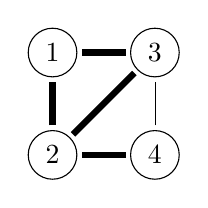
\begin{tikzpicture}[scale=1, every node/.style={circle,draw,minimum size=5mm}]
            \node (n0) at (0,1.3) {1};
            \node (n1) at (0,0) {2};
            \node (n2) at (1.3,1.3) {3};
            \node (n3) at (1.3,0) {4};
            \draw[line width=0.8mm, black] (0,0.375) -- (0,0.93);
            \draw[very thin, black] (1.3,0.375) -- (1.3,0.93);
            \draw[line width=0.8mm, black] (0.375,0) -- (0.93,0);
            \draw[line width=0.8mm, black] (0.375,1.3) -- (0.93,1.3);
            \draw[line width=0.8mm, black] (0.26,0.26) -- (1.04,1.04);
        \end{tikzpicture}
        \caption{\centering Ścieżka nie stanowiąca minimalnego drzewa rozpinającego (4 kroki).}
        \label{fig:minimum_spanning_tree_b}
    \end{subfigure}
    \caption{Ścieżki spełniające oraz nie spełniające założeń \textit{MST} (pogrubione linie).}
    \label{fig:minimum_spanning_tree}
\end{figure}